%%
%% Example UCD Dissertation file
%% Author: Sarah Kreidler
%% Last Updated: 4/13/2014
%%
%% Note, this was generated from the LyX editor, so some commands
%% may not be needed
%%
\documentclass[english]{ucdenver-dissertation}
\usepackage[T1]{fontenc}
\usepackage[latin9]{inputenc}
\usepackage{array}
\usepackage{float}
\usepackage{amsmath}
\usepackage{graphicx}
\usepackage{setspace}
\usepackage[authoryear]{natbib}
\doublespacing

\makeatletter

%%%%%%%%%%%%%%%%%%%%%%%%%%%%%% LyX specific LaTeX commands.
%% Special footnote code from the package 'stblftnt.sty'
%% Author: Robin Fairbairns -- Last revised Dec 13 1996
\let\SF@@footnote\footnote
\def\footnote{\ifx\protect\@typeset@protect
    \expandafter\SF@@footnote
  \else
    \expandafter\SF@gobble@opt
  \fi
}
\expandafter\def\csname SF@gobble@opt \endcsname{\@ifnextchar[%]
  \SF@gobble@twobracket
  \@gobble
}
\edef\SF@gobble@opt{\noexpand\protect
  \expandafter\noexpand\csname SF@gobble@opt \endcsname}
\def\SF@gobble@twobracket[#1]#2{}
%% Because html converters don't know tabularnewline
\providecommand{\tabularnewline}{\\}


%%%%%%%%%%%%%%%%%%%%%%%%%%%%%% User specified LaTeX commands.
%%\newtheorem{thm}{Theorem}
%%\newtheorem{lem}[thm]{Lemma}
%%\newdefinition{rmk}{Remark}
%%\newproof{pf}{Proof}
%%\usepackage{array}
%%\usepackage{ragged2e}
%%\newcolumntype{P}[1]{>{\RaggedLeft\hspace{0pt}}p{#1}}

%%%%%% FRONT MATTER %%%%%%

\title{My Kick-ass Dissertation}
\authorLast{Student}
\authorFirst{Awesome}
\authorMiddle{Q.}
\education{
B.S., Best University Ever, 2001 \\
M.S., Super Cool University, 2005
}
\school{Colorado School of Public Health}
\program{Biostatistics}
\date{2014}
\submitDate{Date-Fran-Approves-Thesis}
\advisor{Bob Q. Advisor}
\advisorTitle{Associate Professor}
\committeeChair{Susie T. Chair}
\committeeMembers{
Larry O. Committee \\
Curly O. Committee \\
Moe O. Committee
}


%% acknowledgement - this is optional
\acknowledgements{I would like to thank the academy for...
}

%% dedication - this is also optional
\dedication{To quokkas, for being the happiest rodent on earth.}

%% sucks this has to be in here, but it's the only way I 
%% could get the latex to work
\preface{
My dissertation is about stuff.  This is the abstract describing that stuff.  Please give
me a Ph.D. already.
}

\usepackage{array}
\renewcommand\arraystretch{0.5}

\makeatother

\usepackage{babel}
\begin{document}

\chapter{INTRODUCTION}

Here is the mind-blowing introduction to my dissertation.  It is so awesome, you had better 
sit down.  Here's some stuff another dude did \citep{article_2007}.

\chapter{INCREDIBLY GREAT PAPER 1%
\footnote{This chapter has been submitted for publication to the Journal of
Something Really Important by Coauthor 1 and Coauthor 2.%
}}


\section{Summary}

So you are not allowed to display an abstract in UCD formatting rules.
If you still want your abstract for each separate paper, you can add a summary
section, like this.

\section{Introduction}

Intro stuff.

\subsection{Notation}

Notation section, because everyone loves math. 

\subsection{New Methods}

Because every Ph.D. wants to make something new and fancy.



\section{Simulation experiment}

Because we love made up data.


\section{Discussion}

Some interpretations that we totally pulled out of our, well you get the point.

\newpage

\chapter{MY SECOND PAPER%
\footnote{This chapter has been submitted for publication to the Journal of Perpretual Rejection
by Coauthor 1, Coauthor2, and Coauthor 3.%
}\label{chap:paper2}}


\section{Summary}

Abstract of paper 2


\section{Introduction}

Wow, look at all the cool stuff I did.  You should really hire me.


\section{Notation}

More cool math.



\section{Simulation study}

Fake data are my favorite kind of data.

\begin{figure}
\begin{centering}
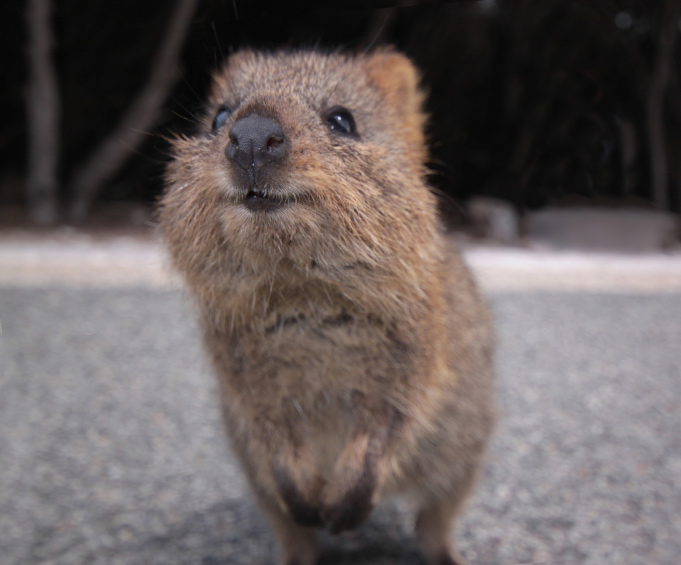
\includegraphics[width=5in]{quokka.jpg}
\par\end{centering}

\caption{Behold! The happy quokka.  Also, notice that Figure captions go below the figure}
\end{figure}

And now, a table.

\begin{table}[H]
\caption{Why quokkas are happier than you (table captions go above the table)}
\begin{centering}
\begin{tabular}{ccc}
\hline 
 & Writing a dissertation?\tabularnewline
\hline 
Quokkas & No\tabularnewline
You & Yes\tabularnewline
\hline 
\end{tabular}
\par\end{centering}

\end{table}

\section{Conclusions}

Seriously, I really need a job and look at all the stuff I just wrote!

\newpage

\chapter{MY THIRD PAPER%
\footnote{This chapter has been submitted for publication to Journal of We Secretly Love Listening 
to Abba, by Coauthor 1, Coauthor 2, Coauthor 3, and Coauthor 4.%
}}


\section{Summary}

Abstract for Paper 3 goes here.


\section{Introduction}

Paper 3 will melt your eyeballs with intellectual glory.





\section{Notation}

I am just going to assume that every dissertation should include math,
because I am a statistician and you should be one too when you grow up.




\section{New Methods}

Here is cool new math that I made up after a caffeine crazed evening
with a multivariate theory book.




\section{Applied example}

Here's how to use my cool methods on real data, because I got bored with 
simulations.  And they take too long to run, anyway.



\section{Discussion}

Don't say I didn't warn you about the eyeball melting thing.

\newpage

\chapter{BIG EPIC CONCLUSION CHAPTER}

OMG, wasn't my dissertation like the coolest thing ever???!!!!


\renewcommand\bibname{REFERENCES}
\singlespacing

\bibliographystyle{ucdDissertation}
\bibliography{example}


\doublespacing

%% had to do some TOC shenanigans, so please use this command instead
%% of regular old \appendix
\ucdappendix

\newpage
\chapter{MIND-ALTERING APPENDIX}

No specific formatting rules for appendices, but make sure it is awesome.  Also, here's an example of the theorem environment.

\section{Theorems}

\begin{theorem}

Some stuff is true. 

\end{theorem} 

\begin{proof}

Because I said so. 
\end{proof}


\end{document}
